\documentclass[a4paper,11pt,twoside,openright]{scrbook}

\usepackage{swThesis}
\usepackage{lipsum}
\usepackage{standalone}
\usepackage{caption}
\standalonetrue

% Bibliography
\bibliography{bibliography}

% Figures
\graphicspath{./figs}

\begin{document}


\chapter{Introduction} \label{chapter:intro}


\section{Eroom's Law: The increasing cost of drug discovery}

Throughout the last 70 years the economic costs of developing novel drugs has increased dramatically, approaching £1 
billion and requiring approximately 10 years from initial concept until regulatory approval.
A study by Scannel \textit{et al.} \cite{Scannell2012} noted that costs approximately double every 9 years, dubbing 
this observation ``Eroom's law'' in a homage to Moore's law. \footnote{The well-known observation that the number of 
transistors in microprocessors approximately doubles every 2 years.}
The reasons behind these ever increasing costs are still under debate, although it is clear the issue is multi-faceted.
One explanation may be that the low-hanging fruits of drug discovery have already been taken, the most effective 
traditional remedies and natural bioactive molecules identified, and their active ingredients commercialised.
As such, whilst many single gene disorders and eminently druggable oncogene-driven homogeneous tumours have been cured, 
the more complex diseases and pharmacological targets remain.
This pessimism has fed the ever present idea that drug discovery is undergoing a productivity crisis, 
\cite{Pammolli2011} and that investments made in early stage research do not translate into actionable pharmacology to 
develop effective therapies, and has led to a renewed interest in alternative drug discovery paradigms.


\section{The drug discovery process}


\subsection{Target-based screening}

Over the past 30 years the majority of drug discovery programmes have seized upon technological advances in robotics 
and automation to screen ever expansive compound libraries against pre-defined protein targets.
It would be difficult to argue that this target-based high-throughput screening (HTS) approach has not been fruitful, 
yielding many successful therapeutics across a range of disease areas, largely attributed to an increased understanding 
of the genomic basis of many diseases.
However, despite numerous clinical and commercial success stories, HTS is not a panacea, with a high attrition rate of 
lead compounds once they enter clinical trials. \cite{Waring2015}
A large majority of these clinical trial failures are not due to toxicity, but rather a lack of efficacy which can 
often be traced back to limited validation of the hypothesised target in the face of complex disease aetiology. 
\cite{Harrison2016}


\subsection{Phenotypic screening}

Phenotypic screening differs from target-based screening in that it does not rely on prior knowledge of a specific 
target, but instead interrogates a biologically relevant assay to identify compounds which alter the phenotype in a 
biologically desirable way.
This target-agnostic approach can prove useful in diseases with poorly understood mechanisms or those with no obvious 
druggable protein targets.
Phenotypic screening is not a new approach in small molecule drug discovery, it was the primary method for many decades 
before the genomics revolution made target hypothesis more tractable.
\cite{Zheng2013}

Many concerns related to phenotypic screening are centred on the lack of mechanistic information for a given lead 
compound.
Whilst the lack of a known target presents challenges and may cause concerns within a commercial drug discovery 
programme, regulatory bodies such as the Food and Drug Administration (FDA) and European Medicines Agency (EMA) do not 
require a known target for drug approval, only that the drug is safe and efficacious.
Metformin is a first-line therapy for type 2 diabetes and is on the World Health Organisation's list of essential 
medicines, it decreases liver glucose production and has an insulin sensitising effect on many tissues.
Despite approval since 1957 and widespread clinical use, the  molecular mechanism of metformin remained unknown for 43 
years. \cite{Hundal2000}
Although knowledge of the molecular target is not necessary to get a drug into the clinic, target deconvolution is 
still an important part of most phenotypic drug discovery programmes, without knowing the protein or proteins a 
compound is binding to, lead optimisation via structure activity relationship (SAR) studies becomes extremely difficult.
In addition, knowledge of the molecular target of a lead compound generated by a phenotypic screen can be used as a 
basis for instigating a conventional high-throughput hypothesis-driven screen on a novel target, this is why many view 
phenotypic screening as a complimentary method to target based screening rather than a competing approach or proposed 
replacement. \cite{Moffat2014}


\section{High content imaging}

High content imaging is a technique utilising high-throughput microscopes and automated image analysis, commonly used 
in phenotypic screening as a method for gathering multivariate datasets from images of biological specimens and has 
proven useful in a wide variety of phenotypic assays, ranging from 2D mammalian cells, \cite{Leggett2016,Tabata2015} 
\textit{in vivo} studies in zebrafish \cite{GeoffreyBurns2005} and even plants and crops. \cite{Chen2014}

High content screens -- screening studies carried out with high content imaging -- are particularly useful in 
phenotypic drug discovery for several reasons.
High content imaging provides spatial resolution enabling the use of more complex assays including co-culture and 3D 
models, which might better represent the biological complexity of disease relative to 2D reductionist models.
However, these complex assays often have phenotypes which are more difficult to quantify, which a single univariate 
readout may fail to accurately recapitulate,
therefore the multivariate datasets produced by high content screening enables a more in-depth view into the endpoints 
which should be measured in a complex assay.
A second benefit is the multivariate data generated by high content screening offers a more unbiased method for 
detecting hits in a phenotypic assay, as predicting which variable to measure beforehand may lead to missed 
biologically interesting phenotypes.
With the advent of more complex datasets generated from high-content imaging, the process of image-analysis and 
computational methods for data processing has given rise to the term ``high-content analysis''.


\subsection{Image analysis}

Image analysis is the process in which raw image data from a high-content screen is transformed into measurements which 
can be used to describe the observed morphology of the biological specimen exposed to a perturbagen.
Here I will focus on cell-based assays for small-molecule screening, though the same methods apply for most other 
assays (spheroids/organoids etc) and perturbagens (siRNA, CRISPR etc).

The standard approach to extracting numerical features from cell morphologies is through segmenting cells and 
sub-cellular structures into ``objects'', and then computing image-based measurements on those objects.
Typically each cell within an image is identified by first segmenting nuclei from the background.
A number of well-established image thresholding algorithms can be used for segmenting nuclei from background, most 
automatically calculate an intensity threshold to binarise an image based on histograms of pixel 
intensities.\cite{Otsu1979,Padmanabhan2010}
The segmented nuclei can then be used as seeds to detect cell boundaries, either through edge detection in a channel 
containing a cytoplasmic marker, or more crudely by expanding a number of pixels from the nuclei centre to approximate 
cell size.
There are also less commonly used methods which utilise machine learning based on trained parameters to segment cells, 
\cite{Sommer2011} or forgo segmentation entirely to measure morphological features from the raw images. 
\cite{Rajaram2012,Orlov2008}

After cells and sub-subcelluar objects have been segmented morphological characteristics are measured for each object, 
these measurements can cover a wide variety of morphologies depending on the aims of the assay, although can be grouped 
into 4 main classes:

\paragraph{Shape.}
Calculated on the properties of the object masks, e.g. area, perimeter, eccentricity. Shape features are commonly used 
as they are interpretable, robust, and quick to calculate.

\paragraph{Intensity.}
These features are based on the pixel intensity values within the object boundaries.
They can be calculated for multiple channels and include measurements such as average intensity, integrated intensity, 
and radial distribution of intensity values.
Great care has to be taken when using intensity values as they are susceptible to batch effects and microscope 
artefacts such as vignetting. \cite{Goldman2010}

\paragraph{Texture.}
Measures of patterns of intensities within objects, typically derived from grey level co-occurrence matrices. 
\cite{Haralick1973} 
This can be used to quantify morphologies such as small speckles or stripes within an image.
Texture measurements are often computationally expensive and difficult to interpret although can be useful for 
measuring subtle morphological changes.

\paragraph{Spatial context.}
These are typically relationships between objects, such as the number of neighbouring cells or nuclei, percentage of a 
cell boundary in contact with neighbouring cells. This class can also include the simple measure of cell or nuclei 
count within a field of view.


\subsection{Data analysis}

Measuring morphological features produces an $m \times n$ dataset per object class, where $m$ is the number of objects 
and $n$ is the number of morphological features measure for that object.
Commonly single object level data is aggregated to population level, where the population can be a field of view, 
microtitre-well, or treatment level (see figure \ref{figure:aggregation}); with the most popular aggregation method 
being a simple median average. \cite{Caicedo2017}
Once the object-level data has been aggregated to a common population level such as per well data, the features from 
each object class can be combined into a dataset represented by a single $p \times q$ matrix, where $p$ is the number 
of wells (or other level of aggregation), and $q$ is the total number of combined features from all object classes.
It is then useful to view each row of this matrix as a feature vector, or morphological profile which summarises the 
morphology induced by a treatment.

\begin{figure}
    \captionsetup{width=0.8\textwidth}
    \caption[Single cell aggregation to a median profile]{Single cell data aggregation to a median profile. Two 
matrices representing single cell morphology data for a treatment, with columns displaying multiple measured 
morphological features for each cell represented as a row. \textit{(Figure re-used from Caicedo et al. Nat Methods, 
2017)}}
    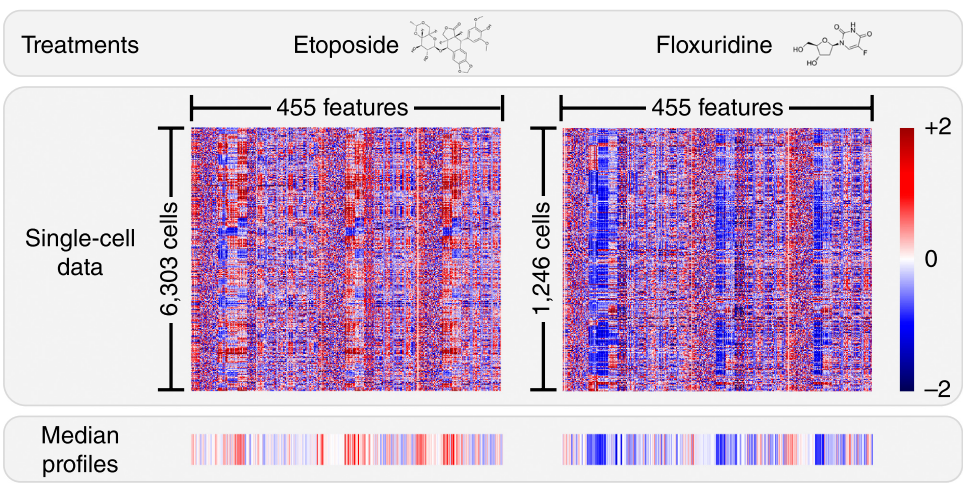
\includegraphics[width=0.8\linewidth]{figs/ch1SingleCellAggregation}
    \label{figure:aggregation}
\end{figure}

There are a number of fairly standard data pre-processing steps involved in high content analysis, consisting of: 
quality-control checks and outlier removal, batch correction, normalisation, standardising feature values, and 
dimensional reduction or feature selection. \cite{Caicedo2017}


\paragraph{Quality control.}
Errors are usually introduced at the imaging or segmentation phase of high-content assays, either through poor image 
quality caused by out-of-focus wells or debris, or poorly chosen segmentation parameters causing artefacts with 
otherwise acceptable images and subsequent outlier morphological features.
As assays often generate thousands if not millions of images, it is not practical to manually check each image and 
segmentation mask for quality, therefore a number of automated methods have been developed to flag potential image 
artefacts and extreme feature values.
Image artefacts can be detected through measures of image intensity, as out-of-focus images tend to have shallow 
intensity gradients across the image and lose high-frequency intensity changes, \cite{Bray2012} whereas images 
containing debris such as dust and fibres contain a large percentage of saturated pixels.
Segmentation errors usually create extreme values for most feature measurements which can be highlighted using typical 
outlier detection methods such as Hampel filtering \cite{Hampel1974} and local outlier factor. \cite{Breunig2000}

\paragraph{Batch correction.}
Batch effects are accumulations of multiple sources of technical variation such as equipment, liquid-handling error, 
reagents and environmental conditions which can influence measurements and mislead researchers, and are particularly 
prevalent in high-throughput experiments.
They are normally identified visually through boxplots of features, with plates or weeks on the x-axis, or through 
comparing correlations, within plates, between plates of the same batch and across batches.
If batch effects are apparent they can be corrected, the simplest method is to standardise each batch separately, other 
methods include 2-way ANOVA \cite{Nygaard2016} or canonical correlation analysis. \cite{Vaisipour2014}

\paragraph{Standardisation.}
When many morphological features are measured from an image, they are unlikely to share the same scale/units or have 
similar variance -- e.g. cell-area measured in pixels which may range from zero to several thousand and 
cell-eccentricity which is constrained between zero and one.
It is therefore useful to standardise all feature values to be mean centred and have comparable variance.
This aids in many downstream data analysis methods which assume standardised feature values.

\paragraph{Dimensional reduction and feature selection.}
As with any high-dimensional data a large number of features can cause issues with analysis and interpretation, this is 
commonly known as the ``curse of dimensionality''. \cite{Bellman1961}
Another issue is that many of the measured features may not contribute information, either as they have little or no 
variation between samples, or are redundant due to high correlation with existing features.
Dimensional reduction and feature selection methods are both commonly used in other biological fields such as genomics 
and proteomics, and are now routinely used in high-content imaging analysis.
A widely used technique is principal component analysis (PCA), which is an unsupervised approach to maximise variation 
through a linear combination of orthogonal features.
PCA can be used to reduce the number of features by selecting a subset of principal components which explain a 
specified proportion of variance in the data.
Loss of interpretability can be an issue when using PCA, and is why some researchers favour feature selection methods 
which aim to retain original feature labels whilst still reducing dimensionality by removing uninformative features.
Many of the feature selection methods are supervised, which may not fit in with unbiased analyses, although Peng 
\textit{et al.} developed an unsupervised minimum-redundancy-maximum-relevancy (mRMR) feature selection method which 
has found use in high-content analyses. \cite{Peng2005}\newline


Following data pre-processing, downstream analysis is typically focused on one of two tasks: identifying hit compounds 
in a screen, or comparing the similarity of morphology profiles created by treatments -- both of which use distance as 
a metric, either comparing hits against a negative control, or treatments against one another respectively.


\subsection{Image based screening}

Phenotypic and image-based screens can be used in traditional drug discovery roles whereby a compound library is 
screened in a biologically relevant cell-based assay in order to identify compounds which produce a favourable 
phenotype and hits or lead compounds identified from a high throughput biochemical assay are evaluated in a more 
complex image-based cell assay to determine their quality.
These assays typically rely on either a positive control compound which is known to elicit the phenotype of interest in 
order to optimise and validate that the assay has appropriate signal-to-noise attributes for testing multiple compounds.
Or alternatively, a carefully designed assay in which a disease model utilising abnormal patient-derived or genetically 
engineered cells is used to identify compounds which revert the disease associated phenotype towards a healthy or 
wild-type phenotype.
An example of this is demonstrated by Gibson \textit{et al.}, \cite{Gibson2015} whereby they modelled cerebral 
cavernous malformation (CCM) using siRNA knockdown of the \textit{CCM2} gene in human primary cells, and screened small 
molecules to identify candidates which rescued the siRNA induced phenotype using fluorescent markers of the nucleus, 
actin filaments, and VE-cadherin cell-cell junctions.
Candidate compounds were then validated in an \textit{in vivo} mouse model, which lead to the ongoing pre-clinical 
development of 4-Hydroxy-TEMPO as a novel therapeutic for CCM.
This is an elegant demonstration that combining good disease models with target agnostic phenotypic screens can 
effectively yield promising therapeutic candidates without complex bioinformatics techniques.


\subsection{Image based profiling}

In contrast to screening studies which are mainly interested in looking for a defined phenotype, profiling is used to 
create phenotypic ``fingerprints'' of perturbagens analogous to transcriptional profiles, which can be used for 
clustering, inference and prediction.
One of the main uses of phenotypic profiling is to compare the similarity of morphological profiles allowing clustering 
and machine learning methods to build rules in order to classify new or blinded treatments according to similar 
annotated neighbouring treatments.

One of the landmark papers of high-content profiling was published in 2004 when Perlman \textit{et al.} 
\cite{Perlman2004a} first demonstrated that morphological profiles between drugs could be clustered according to 
compound mechanism-of-action using a custom similarity metric and hierarchical clustering.
Most studies utilising morphological profiling use unsupervised hierarchical clustering in order to group treatments 
into bins which produce similar cellular phenotypes, \cite{Gustafsdottir2013,Young2008} although other clustering 
algorithms such as graph-based Markov clustering algorithm (MCL), \cite{Reisen2015,VanDongen2008} and spanning trees 
\cite{Qiu2011} are sometimes used.


\section{Phenotypic screening in cancer drug discovery}

Cancer drug discovery programmes of past decades seized upon uncontrolled proliferation as a clinically relevant 
phenotype to use in screening studies, giving rise to a number of anti-proliferative and cytotoxic compounds, which are 
still used in the clinic but often renowned for their severe side-effects.
Many modern day oncology drug discovery programmes still retain anti-proliferation as a key predictor for pre-clinical 
success, although increased understanding of cancer's molecular underpinnings has driven many oncology programmes 
towards a more target-directed approach.
The prototypical success story of target-driven drug discovery in oncology is imatinib, a tyrosine kinase inhibitor 
targeting the BCR-ABL fusion protein in chronic myeloid leukemia.
However, despite imatinib's exceptional success, unfortunately in most cases targeting a single driver in a complex 
signalling network results in compensatory signalling, activation of redundant pathways and unpredicted feedback 
mechanisms, all of which diminish efficacy \textit{in vivo}.

In a review of 48 small molecule drugs approved for use in oncology between 1999 and 2013, $31/48$ were discovered 
through target based screens, whereas $17/48$ were based on leads from target-agnostic phenotypic screens, 
\cite{Moffat2014} of those compounds discovered through target directed screening programmes the vast majority (75\%) 
were kinase inhibitors.
However, phenotypically derived compounds did not live up to the hypothesis that target-agnostic screening should be 
more likely to identify compounds with novel MoAs, \cite{Swinney2011} with only $5/17$ being first in class molecules.
An explanation for this sparsity of novel mechanisms is that phenotypic assays which use cytotoxicity readouts are 
likely to find low-hanging fruit such as targeting microtubule stabilisation and DNA replication dynamics. 
\cite{Moffat2014}
One option to combat this narrow attention on a select few targets -- caused by either hypothesis-driven or simplistic 
phenotypic screens -- is to utilise the more detailed mechanistic information offered by high-content imaging to 
explore novel biological mechanism and thus broader areas of therapeutic target space rather than relying on cellular 
death as catch-all phenotypic readout.

In addition to high-content imaging screens with cells grown in 2D monolayers, more complex phenotypic models such as 
3D tumour spheroids are being increasingly adopted in pre-clinical oncology.
3D tumour spheroids are multi-cellular aggregates thought to better recapitulate environment and biology of real 
tumours compared to cells grown in 2D monolayers on tissue culture plastic.
There is mounting evidence that spheroids offer a more predictive model of \textit{in vivo} compound efficacy than 
their 2D counterparts, \cite{Pickl2009, Breslin2013,Lovitt2013} this is thought to be caused by the hypoxic environment 
in the centre of the spheroid, increased cell-cell contact and greater presence of extracellular matrix components 
which better represents conditions found \textit{in vivo}.
Three-dimensional spheroid models lend themselves well to phenotypic and image-based screening projects, with compound 
efficacy determined through use of fluorescent markers of cell-viability, \cite{Lovitt2013} cell-cycle dynamics, 
\cite{Laurent2013} or by analysis of spheroid morphology which can also incorporate 3D volumetric measurements. 
\cite{Huang2017}


\subsection{Cancer cell line panels}

Panels of multiple cancer cell lines such as the NCI-60, Cancer Cell Line Encyclopedia (CCLE) \cite{Barretina2012} and 
Genomics of Drug Sensitivity in Cancer (GDSC) \cite{Yang2013} have been widely used to facilitate high-throughput 
screening and increase certainty in hit selection / disease-specificity,\cite{Wu1992,Shoemaker2006} and as a research 
tool to study pharmacogenomics. \cite{Heiser2012,Abaan2013,Jaeger2015}
The use of cancer cell line panels can also benefit phenotypic screens by mirroring the heterogeneity found in patient 
populations, as well as heterogeneous cell populations found in tumours. \cite{Caie2010}
Throughout this body of work I have used a panel of eight breast cancer cell lines (table \ref{table:cell-lines} and 
figure \ref{figure:cell_images} A), these cell lines were chosen based on a number of criteria:
\begin{enumerate}
    \item Relatively fast growth to allow compound screening to be performed in weekly batches.
    \item Adherent to tissue culture plastic to enable 2D imaging.
    \item Form a monolayer when grown in 2D -- overlapping cells cause difficulties for most image segmentation methods.
    \item Amenable for morphometric imaging -- larger and/or flatter cells allow for better discrimination of 
sub-cellular features.
    \item Distinct morphologies to evaluate the robustness of morphological profiling methods.
    \item A collection which represents a range of molecular sub-classes of breast cancer.
\end{enumerate}

\begin{table}[]
    \begin{footnotesize}
    \captionsetup{width=0.8\linewidth}
    \centering
    \caption[Panel of breast cancer cell lines chosen for study]{Panel of breast cancer cell lines chosen for study. 
PI3K:Phosphoinsitide-3-kinase, PTEN:Phosphatase and tensin homolog, ER:Estrogen receptor, TN:triple-negative, 
HER2:human epidermal growth factor, WT:wild-type, $\star$:lack of consensus regarding the mutational status.}
    \label{table:cell-lines}
    \begin{tabular}{@{}llll@{}}
    \toprule
               &                    & \multicolumn{2}{l}{Mutational status} \\
    Cell line  & Molecular subclass & PTEN             & PI3K               \\ \midrule
    MCF7       & ER                 & WT               & E545K              \\
    T47D       & ER                 & WT               & H1047R             \\
    MDA-MB-231 & TN                 & WT               & WT                 \\
    MDA-MB-157 & TN                 & WT               & WT                 \\
    HCC1569    & HER2               & WT               & WT                 \\
    SKBR3      & HER2               & WT               & WT                 \\
    HCC1954    & HER2               & $\star$          & H1047R             \\
    KPL4       & HER2               & $\star$          & H1047R             \\ \bottomrule
    \end{tabular}
    \end{footnotesize}
\end{table}

\begin{figure}
    \centering
    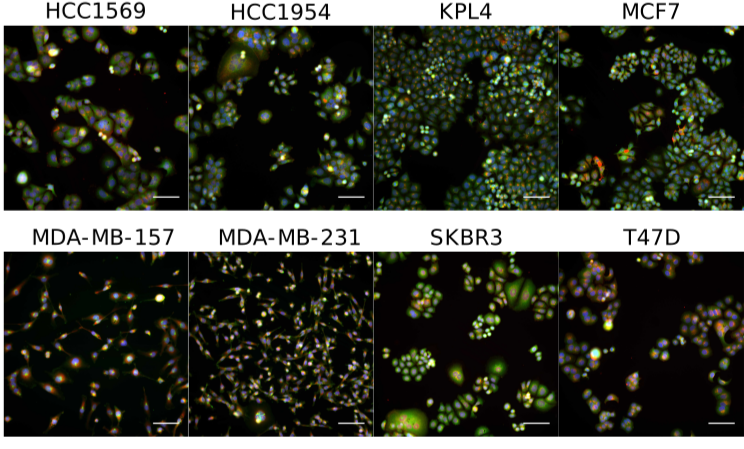
\includegraphics[width=0.8\textwidth]{ch1cellImage}
    \captionsetup{width=0.8\textwidth}
    \caption[Images of the eight breast cancer cell-lines]{
        Composite image of cell-lines treated with 0.1\% DMSO showing distinct morphology between untreated cell-lines.
        Channels used: Red - MitoTracker DeepRed; Green - Concanavalin A; Blue - Hoechst33342. Scale bars: 100 $\mu$m.
    }
    \label{figure:cell_images}
\end{figure}


\subsection{Breast cancer}

The cell lines used in this work are all immortalised human cancer cell lines originating from breast cancer patients.
Breast cancer cell lines were chosen as the disease has been the focus of many years of research resulting in many well 
characterised cell lines with freely available genomic, proteomic and imaging datasets.
Breast cancer is sub-divided into several sub-classes defined by the molecular components which drive disease 
progression.
The three main drivers of breast cancer are oestrogen receptor (ER), progesterone receptor (PR), and human epidermal 
growth factor receptor 2 (HER2).
Aberrant signalling in one or more of these pathways is responsible for approximately 80-85\% cases of breast cancer.
The remaining 15-20\% of cases are classified as triple negative (TN).
Molecular sub-classes are used clinically to stratify patients based on immunohistochemically stained tumour sections 
examined by pathologists to inform therapeutic and surgical options.
In addition to these simple subtypes, there are alternative and more complex methods of stratifying patients based on 
histopathological phenotype, response to endocrine and (neo)adjuvant therapy, and copy number alterations. 
\cite{Sims2007}


\section{Hypothesis, general aims and thesis structure}

As has already been discussed, image-based screens can generate large multivariate datasets which differ considerably 
from those usually found in high-throughput screening environments, the work in this thesis aims to address the 
hypothesis that informatics tools can be better utilised in the context of high-content screening in cancer drug 
discovery.
This work aims to generate new high-content screening datasets across a panel of breast cancer cell-lines with which to 
compare, investigate and develop new data-analysis tools to better leverage the data present -- as well as how best to 
combine this high-content imaging data with existing biological and chemical databases to better lead and inform 
early-stage drug discovery programmes.

The following chapters focus on selected topics from my PhD, some of the work has been previously published (see 
appendix).

\begin{itemize}
\item Chapter \ref{chapter:generalMethods} contains general methods which are used throughout and apply to multiple 
chapters.
\item Chapter \ref{chapter:moa} is an analysis of machine learning methods to classify compound MoA from high content 
imaging data, with a focus on how well classifiers transfer across to new data from morphologically distinct cell lines.
\item Chapter \ref{chapter:tccs} describes the development and application of a novel analytical method to detect and 
quantify differential phenotypic responses between morphologically distinct cell lines when treated with small 
molecules.
\item Chapter \ref{chapter:screen} describes a high content screen of 1280 approved small molecules in order to 
identify compounds which produced distinct phenotypic responses between cell lines, functional assays to validate hits 
and proteomics to investigate potential pathways responsible.
\item Chapter \ref{chapter:cheminformatics} describes work towards developing methods which combine cheminformatics of 
compound chemical structure with high content morphological data in order to infer MoA of unannotated compounds, as 
well as assess the correlation of chemical similarity and phenotypic similarity.
\item Chapter \ref{chapter:discussionAndConclusion} presents concluding remarks about my work and future directions for 
the field.
\end{itemize}


\end{document}
